\documentclass{article}
\usepackage[utf8]{inputenc}

\author{Ryhmä 5}
\title{Verkkosivut yritykselle\\
\large Suunnitteludokumentti}


\begin{document}
\maketitle
\section{Johdanto}
Projektimme tavoitteena on suunnitella ja toteuttaa yritykselle konseptimalli verkkosivustosta, joka sisältää verkkokaupan. Pääpaino on verkkokaupan
toiminnoissa, koska se vaatii eniten osaamista koko fullstack-kirjolla. Projekti voidaan jakaa osiin, ohjelmointikielien mukaan. HTML määrittelee verkkosivun rakenteen,
CSS ulkoasun, JavaScript toiminnallisuudet käyttäjälaitteen puolella, PHP palvelimen toiminnallisuudet ja SQL tietokannan.

\section{Määrittely}
\subsection{HTML}
Verkkosivusto rakentuu kolmesta eri sivusta, etusivusta, joka sisältää myös verkkokaupan, yrityksen infosivusta ja yhteystietosivusta. Kullekin sivulle yhteisiä elementtejä ovat yläosan navigaatiopalkki, sekä alaosan infolaatikko.

\subsection{CSS}
Koko sivusto käyttää yhtä CSS-tiedostoa, jolla saadaan yhtenäinen, sivustonlaajuinen ulkoasu.

\subsection{JavaScript}
JavaScript kuuntelee asiakkaan komentoja ja käsittelee ne, esimerkiksi lähettäen kutsun palvelimelle, tai päivittämällä sivun hakuehtojen mukaiseksi.
\subsection{PHP}
PHP käsittelee asiakkaan pyynnöt, tekee palvelinpuolen tietokantakutsut ja palauttaa ne asiakkaalle.
\subsection{SQL}
SQL-tietokanta sisältää verkkokaupan tuotteet, rekisteröidyt asiakkaat ja tilaukset.

\section{Asiakaskokemukset}

\begin{itemize}
    \item Asiakas voi etsiä tuotetta hakusanalla, kategorialla tai tuotetunnuksella.
    \item Asiakas voi järjestää hakutulokset aakkosittain tai hinnan mukaan.
    \item Asiakas voi ostaa yhden tai useamman tuotteen verkkokaupasta.
\end{itemize}

\section{Käyttötapauskaavio}

\end{document}



\documentclass{article}
\usepackage[utf8]{inputenc}
\usepackage{graphicx}
\usepackage{geometry}
\usepackage{hyperref}

\author{Ryhmä 5}
\title{Verkkosivut yritykselle\\
\large Suunnitteludokumentti}


\begin{document}
\maketitle
\section{Johdanto}
Projektimme tavoitteena on suunnitella ja toteuttaa yritykselle konseptimalli verkkosivustosta, joka sisältää verkkokaupan. Pääpaino on verkkokaupan
toiminnoissa, koska se vaatii eniten osaamista koko fullstack-kirjolla. Projekti voidaan jakaa osiin, ohjelmointikielien mukaan. HTML määrittelee verkkosivun rakenteen,
CSS ulkoasun, JavaScript toiminnallisuudet käyttäjälaitteen puolella, PHP palvelimen toiminnallisuudet ja SQL tietokannan.

\section{Määrittely}
\subsection{HTML}
Verkkosivusto rakentuu kolmesta eri sivusta, etusivusta, joka sisältää myös verkkokaupan, yrityksen infosivusta ja yhteystietosivusta. Kullekin sivulle yhteisiä elementtejä ovat yläosan navigaatiopalkki, sekä alaosan infolaatikko.

\subsection{CSS}
Koko sivusto käyttää yhtä CSS-tiedostoa, jolla saadaan yhtenäinen, sivustonlaajuinen ulkoasu.

\subsection{JavaScript}
JavaScript kuuntelee asiakkaan komentoja ja käsittelee ne, esimerkiksi lähettäen kutsun palvelimelle, tai päivittämällä sivun hakuehtojen mukaiseksi.
\subsection{PHP}
PHP käsittelee asiakkaan pyynnöt, tekee palvelinpuolen tietokantakutsut ja palauttaa ne asiakkaalle.
\subsection{SQL}
SQL-tietokanta sisältää verkkokaupan tuotteet, rekisteröidyt asiakkaat ja tilaukset. Lisäksi varastotaulu sisältää tuotemäärät. Tämä taulu voidaan varmuuskopioida määräajoin, jolloin esimerkiksi palvelimen äkillisen kaatumisen aiheuttamat ongelmat voidaan minimoida.

\begin{figure}
    \centering
    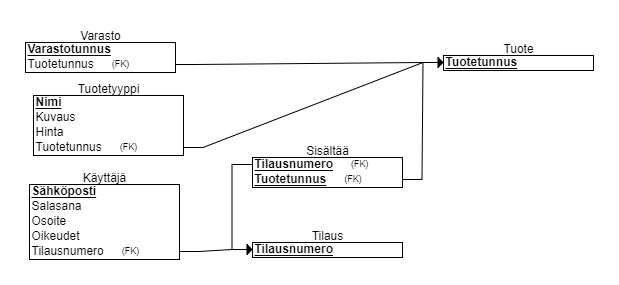
\includegraphics[width=\textwidth]{kuvat/ER-kaavio_oy-ab.png}
    \caption{ER-kaavio}
    \label{fig:er-kaavio}
\end{figure}

\section{Asiakaskokemukset}

\begin{itemize}
    \item Asiakas voi etsiä tuotetta hakusanalla, kategorialla tai tuotetunnuksella.
    \item Asiakas voi järjestää hakutulokset aakkosittain tai hinnan mukaan.
    \item Asiakas voi ostaa yhden tai useamman tuotteen verkkokaupasta.
\end{itemize}
Kuva \ref{fig:userkaavio} näyttää toiminnot kaaviossa. 

Ylläpitäjä voi hyväksyä tilaukset, lisätä tai poistaa tuotteita varastosta, sekä lisätä, päivittää tai poistaa tuotetyyppejä. Asiakkaalla ei tule olemaan ylläpitäjän oikeuksia.

\section{Tietoturva}

Pyrimme turvautumaan ulkopuoliselta vaikuttamiselta sekä virhetilanteilta erilaisilla toimilla, joita ovat muun muassa:

\begin{itemize}
    \item SQL-kutsujen sanitointi.
    \item Käyttäjäautentikoinnin turvallinen toteutus.
    \item Varmuuskopiointi.
    \item Varautuminen XSS-hyökkäyksiin.
    \item Ylläpitäjäoikeuksien turvaaminen.
\end{itemize}


\begin{figure}[h]
    \centering
   \includegraphics[width=\textwidth]{kuvat/userkaavio.png}
    \caption{Käyttötapauskaavio}
    \label{fig:userkaavio}
\end{figure}
\newpage
\section{Projektitiedot}

Ryhmän  5 jäsenet
\begin{itemize}
    \item Joonas Taivalmaa
    \item Eelis Melto
    \item Petteri Piipponen
\end{itemize}

Tämän dokumentin uusin versio löytyy aina GitHubista.

GitHub: \url{http://github.com/joonaset/oy-ab}


\end{document}
